\documentclass{tufte-handout}

\title{Hash Functions }

\author[Packer]{Success Academy High School of the Liberal Arts\\Dr. Anthony Schultz}

\date{September 15 2016} % without \date command, current date is supplied

%\geometry{showframe} % display margins for debugging page layout

\usepackage{graphicx} % allow embedded images
  \setkeys{Gin}{width=\linewidth,totalheight=\textheight,keepaspectratio}
  \graphicspath{{graphics/}} % set of paths to search for images
\usepackage{amsmath}  % extended mathematics
\usepackage{booktabs} % book-quality tables
\usepackage{units}    % non-stacked fractions and better unit spacing
\usepackage{multicol} % multiple column layout facilities
\usepackage{lipsum}   % filler text
\usepackage{fancyvrb} % extended verbatim environments
  \fvset{fontsize=\normalsize}% default font size for fancy-verbatim environments
  \usepackage{mathtools}
  
  
    %MADNESS
  
  \usepackage[T1]{fontenc} % Use 8-bit encoding that has 256 glyphs
\usepackage{fourier} % Use the Adobe Utopia font for the document - comment this line to return to the LaTeX default
\usepackage[english]{babel} % English language/hyphenation
\usepackage{amsmath,amsfonts,amsthm} % Math packages
\usepackage{mathtools}% http://ctan.org/pkg/mathtools
\usepackage{etoolbox}% http://ctan.org/pkg/etoolbox
\usepackage{lipsum} % Used for inserting dummy 'Lorem ipsum' text into the template
\usepackage{units}% To use \nicefrac
\usepackage{cancel}% To use \cancel
%\usepackage{physymb}%To use r
\usepackage{sectsty} % Allows customizing section commands
\usepackage[dvipsnames]{xcolor}
\usepackage{pgf,tikz}%To draw 
\usepackage{pgfplots}%To draw 
\usetikzlibrary{shapes,arrows}%To draw 
\usetikzlibrary{patterns,fadings}
 \usetikzlibrary{decorations.pathreplacing}%To draw curly braces 
 \usetikzlibrary{snakes}%To draw 
 \usetikzlibrary{spy}%To do zoom-in
 \usepackage{setspace}%Set margins and such
 %\usepackage{3dplot}%To draw in 3D
\usepackage{framed}%To get shade behind text


\definecolor{shadecolor}{rgb}{0.9,0.9,0.9}%setting shade color
\allsectionsfont{\centering \normalfont\scshape} % Make all sections centered, the default font and small caps
  
  

  
  

% Standardize command font styles and environments
\newcommand{\doccmd}[1]{\texttt{\textbackslash#1}}% command name -- adds backslash automatically
\newcommand{\docopt}[1]{\ensuremath{\langle}\textrm{\textit{#1}}\ensuremath{\rangle}}% optional command argument
\newcommand{\docarg}[1]{\textrm{\textit{#1}}}% (required) command argument
\newcommand{\docenv}[1]{\textsf{#1}}% environment name
\newcommand{\docpkg}[1]{\texttt{#1}}% package name
\newcommand{\doccls}[1]{\texttt{#1}}% document class name
\newcommand{\docclsopt}[1]{\texttt{#1}}% document class option name
\newenvironment{docspec}{\begin{quote}\noindent}{\end{quote}}% command specification environment

\begin{document}

\maketitle% this prints the handout title, author, and date
\marginnote[-80pt]{Project folder available at: \\ \href{url}{https://github.com/Trismeg/Success}}


\begin{marginfigure}[-40 pt]%
  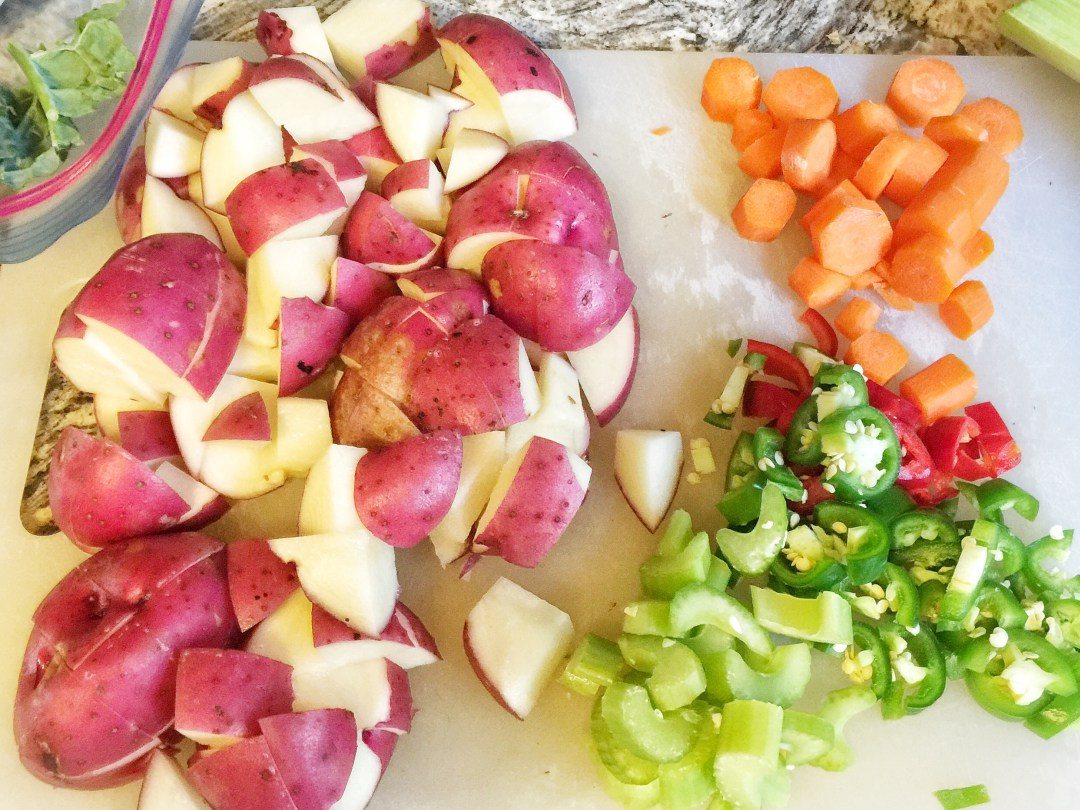
\includegraphics[width=\linewidth]{hash.jpg}
  \caption{Breakfast hash }
  \label{fig:marginfig}
\end{marginfigure}

\marginnote[20pt]{
The word \textbf{hash} entered English in the mid 1600's, during the dawn of science.  It meant \textit{to chop into small pieces} and represented a brilliant culinary advancement.  It came from the French \textbf{\textit{hacher}}, \textit{chop up}.  This deriving from Old French \textbf{\textit{hache}}, \textit{ax}.}


\begin{abstract}
\noindent
This is an introduction to one of the most fundamental tools in modern cryptography, hash functions.  Hash functions are awesome because they secure global digital communications and make amazing things possible.   Today we will do the following: 
\begin{itemize}
\item learn what is a hash function and its properties
\item learn how to compute a hash function
 \item imagine useful applications of hash functions
 \end{itemize} \end{abstract}

\normalsize

\begin{marginfigure}[10 pt]%
  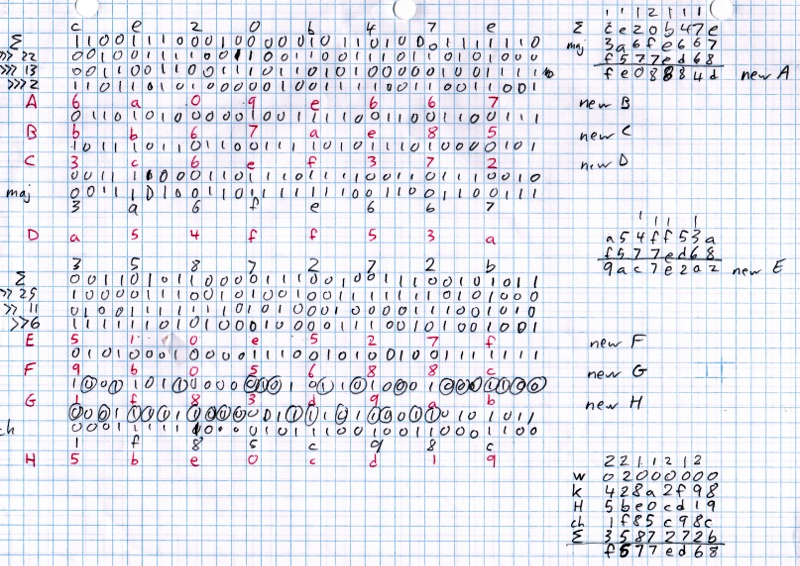
\includegraphics[width=\linewidth]{sha.jpg}
  \caption{Hashing with SHA-256 by hand: www.youtube.com/watch?v=y3dqhixzGVo}
  \label{fig:marginfig}
\end{marginfigure}

\section{Expectations}
During this lesson students are expected to do the following. 
\begin{itemize}
\item direct attention toward the subject of hashing with laser-like precision \\(\textbf{no talking to neighbors})
\item use only the indicated computing utilities while using the computer \\(\textbf{no texting or snapchatting grandma})
 \item muster deep intellectual enthusiasm for the tasks at hand\\ (\textbf{participate fully})
 \end{itemize}

\section{Hash Functions}

Hashing is something we do to data/numbers which adds randomness.  A hash function, $H$, takes input data called a \textbf{message}, m, and outputs data called a \textbf{digest}, d.  

\marginnote[20pt]{Using function notation from mathematics we can describe a hash function $H$ taking an input message $m$ and output digest $d$.

$$H(m)\longrightarrow d$$

\textbf{Feature 1}: We should not be able to get input $m$ from output $d$.  A hash function should have no inverse.
$$ m\mathrlap{\longleftarrow}{\ \ \Large \times}\ \  H^{-1}(d)$$
\textbf{Feature 2}: A hash function should be so random that changing one little thing in $m$ completely changes $d$.\\
\textbf{Feature 3}: It should be impossible to find two different input $m$ values which give the same output $d$ values.  This is called a collision and it is BAD!!! 
$$ H(m_1)\mathrlap{\longleftrightarrow}{\ \ \Large \times}\ \  H(m_2)$$}

\subsection{Features}
A good hash function should be straightforward to use and have the three following features.
\begin{enumerate}
\item{It is physically infeasible to determine an input message from its output hash value.}  
\item{Any change to the input message should change the output has value so extensively as to make it appear uncorrelated to the old hash value.}
\item{It is physically infeasible to find two different input messages with the same output hash values.}
\end{enumerate}

\newpage
\section{How to Hash}
\marginnote[20pt]{Hexadecimal or hex numbers are base 16.  In our day to day lives we use base 10 numbers.  The numerals for hexadecimal numbers are written:
$$\texttt{01234567890abdef}$$}
The easiest way to get started hashing is to visit the following website.\\ \ \\
\href{url}{www.fileformat.info/tool/hash.htm} \\ \ \\
\noindent The website will compute various hash digests in hexidecimal (base 16).

\section{Activity}
\noindent Go to the website and hash the word "Hello".  \\ \ \\

\textbf{Complete the following:}
\begin{enumerate}
\item{How many different kinds of hash digests does the website compute?}\\  
\item{Write down the Adler32 digest of the word "Hello". }\\
\item{Write down the Adler32 digest of the word "hello". }\\
\item{Explain which feature of hash functions requires the digest of "Hello" and "hello" to be totally different.}\\ \vspace{1cm}
\item{Is there another word (string) that has the same Adler32 digest of the word "Hello"?\\ \vspace{2cm}  If so, how could we find it?\\ \vspace{2cm}  How hard would it be to find it?} \\ \vspace{2cm}
\item{What would be the use of taking a hash digest of a 3D printer .STL file?}
\end{enumerate}



%\bibliography{sample-handout}
%\bibliographystyle{plainnat}



\end{document}
